\documentclass{ximera}

\outcome{Find the derivative $\frac{dy}{dx}$ for a curve defined parametrically.}
\outcome{Find the equation of a tangent line for a curve defined parametrically.}
\outcome{Find where a parametrically defined curve has vertical and horizontal tangent lines.}
\outcome{Understand the difference between a curve and the representation of the curve.}


%\usepackage{todonotes}

\newcommand{\todo}{}

\usepackage{esint} % for \oiint
\ifxake%%https://math.meta.stackexchange.com/questions/9973/how-do-you-render-a-closed-surface-double-integral
\renewcommand{\oiint}{{\large\bigcirc}\kern-1.56em\iint}
\fi


\graphicspath{
  {./}
  {ximeraTutorial/}
  {basicPhilosophy/}
  {functionsOfSeveralVariables/}
  {normalVectors/}
  {lagrangeMultipliers/}
  {vectorFields/}
  {greensTheorem/}
  {shapeOfThingsToCome/}
  {dotProducts/}
  {partialDerivativesAndTheGradientVector/}
  {../productAndQuotientRules/exercises/}
  {../normalVectors/exercisesParametricPlots/}
  {../continuityOfFunctionsOfSeveralVariables/exercises/}
  {../partialDerivativesAndTheGradientVector/exercises/}
  {../directionalDerivativeAndChainRule/exercises/}
  {../commonCoordinates/exercisesCylindricalCoordinates/}
  {../commonCoordinates/exercisesSphericalCoordinates/}
  {../greensTheorem/exercisesCurlAndLineIntegrals/}
  {../greensTheorem/exercisesDivergenceAndLineIntegrals/}
  {../shapeOfThingsToCome/exercisesDivergenceTheorem/}
  {../greensTheorem/}
  {../shapeOfThingsToCome/}
  {../separableDifferentialEquations/exercises/}
}

\newcommand{\mooculus}{\textsf{\textbf{MOOC}\textnormal{\textsf{ULUS}}}}

\usepackage{tkz-euclide}\usepackage{tikz}
\usepackage{tikz-cd}
\usetikzlibrary{arrows}
\tikzset{>=stealth,commutative diagrams/.cd,
  arrow style=tikz,diagrams={>=stealth}} %% cool arrow head
\tikzset{shorten <>/.style={ shorten >=#1, shorten <=#1 } } %% allows shorter vectors

\usetikzlibrary{backgrounds} %% for boxes around graphs
\usetikzlibrary{shapes,positioning}  %% Clouds and stars
\usetikzlibrary{matrix} %% for matrix
\usepackage{pgfplots}
\usepgfplotslibrary{polar} %% for polar plots
\usepgfplotslibrary{fillbetween} %% to shade area between curves in TikZ
\usetkzobj{all}
\usepackage[makeroom]{cancel} %% for strike outs
%\usepackage{mathtools} %% for pretty underbrace % Breaks Ximera
%\usepackage{multicol}
\usepackage{pgffor} %% required for integral for loops



%% http://tex.stackexchange.com/questions/66490/drawing-a-tikz-arc-specifying-the-center
%% Draws beach ball
\tikzset{pics/carc/.style args={#1:#2:#3}{code={\draw[pic actions] (#1:#3) arc(#1:#2:#3);}}}



\usepackage{array}
\setlength{\extrarowheight}{+.1cm}
\newdimen\digitwidth
\settowidth\digitwidth{9}
\def\divrule#1#2{
\noalign{\moveright#1\digitwidth
\vbox{\hrule width#2\digitwidth}}}





\newcommand{\RR}{\mathbb R}
\newcommand{\R}{\mathbb R}
\newcommand{\N}{\mathbb N}
\newcommand{\Z}{\mathbb Z}

\newcommand{\sagemath}{\textsf{SageMath}}


%\renewcommand{\d}{\,d\!}
\renewcommand{\d}{\mathop{}\!d}
\newcommand{\dd}[2][]{\frac{\d #1}{\d #2}}
\newcommand{\pp}[2][]{\frac{\partial #1}{\partial #2}}
\renewcommand{\l}{\ell}
\newcommand{\ddx}{\frac{d}{\d x}}

\newcommand{\zeroOverZero}{\ensuremath{\boldsymbol{\tfrac{0}{0}}}}
\newcommand{\inftyOverInfty}{\ensuremath{\boldsymbol{\tfrac{\infty}{\infty}}}}
\newcommand{\zeroOverInfty}{\ensuremath{\boldsymbol{\tfrac{0}{\infty}}}}
\newcommand{\zeroTimesInfty}{\ensuremath{\small\boldsymbol{0\cdot \infty}}}
\newcommand{\inftyMinusInfty}{\ensuremath{\small\boldsymbol{\infty - \infty}}}
\newcommand{\oneToInfty}{\ensuremath{\boldsymbol{1^\infty}}}
\newcommand{\zeroToZero}{\ensuremath{\boldsymbol{0^0}}}
\newcommand{\inftyToZero}{\ensuremath{\boldsymbol{\infty^0}}}



\newcommand{\numOverZero}{\ensuremath{\boldsymbol{\tfrac{\#}{0}}}}
\newcommand{\dfn}{\textbf}
%\newcommand{\unit}{\,\mathrm}
\newcommand{\unit}{\mathop{}\!\mathrm}
\newcommand{\eval}[1]{\bigg[ #1 \bigg]}
\newcommand{\seq}[1]{\left( #1 \right)}
\renewcommand{\epsilon}{\varepsilon}
\renewcommand{\phi}{\varphi}


\renewcommand{\iff}{\Leftrightarrow}

\DeclareMathOperator{\arccot}{arccot}
\DeclareMathOperator{\arcsec}{arcsec}
\DeclareMathOperator{\arccsc}{arccsc}
\DeclareMathOperator{\si}{Si}
\DeclareMathOperator{\scal}{scal}
\DeclareMathOperator{\sign}{sign}


%% \newcommand{\tightoverset}[2]{% for arrow vec
%%   \mathop{#2}\limits^{\vbox to -.5ex{\kern-0.75ex\hbox{$#1$}\vss}}}
\newcommand{\arrowvec}[1]{{\overset{\rightharpoonup}{#1}}}
%\renewcommand{\vec}[1]{\arrowvec{\mathbf{#1}}}
\renewcommand{\vec}[1]{{\overset{\boldsymbol{\rightharpoonup}}{\mathbf{#1}}}}
\DeclareMathOperator{\proj}{\mathbf{proj}}
\newcommand{\veci}{{\boldsymbol{\hat{\imath}}}}
\newcommand{\vecj}{{\boldsymbol{\hat{\jmath}}}}
\newcommand{\veck}{{\boldsymbol{\hat{k}}}}
\newcommand{\vecl}{\vec{\boldsymbol{\l}}}
\newcommand{\uvec}[1]{\mathbf{\hat{#1}}}
\newcommand{\utan}{\mathbf{\hat{t}}}
\newcommand{\unormal}{\mathbf{\hat{n}}}
\newcommand{\ubinormal}{\mathbf{\hat{b}}}

\newcommand{\dotp}{\bullet}
\newcommand{\cross}{\boldsymbol\times}
\newcommand{\grad}{\boldsymbol\nabla}
\newcommand{\divergence}{\grad\dotp}
\newcommand{\curl}{\grad\cross}
%\DeclareMathOperator{\divergence}{divergence}
%\DeclareMathOperator{\curl}[1]{\grad\cross #1}
\newcommand{\lto}{\mathop{\longrightarrow\,}\limits}

\renewcommand{\bar}{\overline}

\colorlet{textColor}{black}
\colorlet{background}{white}
\colorlet{penColor}{blue!50!black} % Color of a curve in a plot
\colorlet{penColor2}{red!50!black}% Color of a curve in a plot
\colorlet{penColor3}{red!50!blue} % Color of a curve in a plot
\colorlet{penColor4}{green!50!black} % Color of a curve in a plot
\colorlet{penColor5}{orange!80!black} % Color of a curve in a plot
\colorlet{penColor6}{yellow!70!black} % Color of a curve in a plot
\colorlet{fill1}{penColor!20} % Color of fill in a plot
\colorlet{fill2}{penColor2!20} % Color of fill in a plot
\colorlet{fillp}{fill1} % Color of positive area
\colorlet{filln}{penColor2!20} % Color of negative area
\colorlet{fill3}{penColor3!20} % Fill
\colorlet{fill4}{penColor4!20} % Fill
\colorlet{fill5}{penColor5!20} % Fill
\colorlet{gridColor}{gray!50} % Color of grid in a plot

\newcommand{\surfaceColor}{violet}
\newcommand{\surfaceColorTwo}{redyellow}
\newcommand{\sliceColor}{greenyellow}




\pgfmathdeclarefunction{gauss}{2}{% gives gaussian
  \pgfmathparse{1/(#2*sqrt(2*pi))*exp(-((x-#1)^2)/(2*#2^2))}%
}


%%%%%%%%%%%%%
%% Vectors
%%%%%%%%%%%%%

%% Simple horiz vectors
\renewcommand{\vector}[1]{\left\langle #1\right\rangle}


%% %% Complex Horiz Vectors with angle brackets
%% \makeatletter
%% \renewcommand{\vector}[2][ , ]{\left\langle%
%%   \def\nextitem{\def\nextitem{#1}}%
%%   \@for \el:=#2\do{\nextitem\el}\right\rangle%
%% }
%% \makeatother

%% %% Vertical Vectors
%% \def\vector#1{\begin{bmatrix}\vecListA#1,,\end{bmatrix}}
%% \def\vecListA#1,{\if,#1,\else #1\cr \expandafter \vecListA \fi}

%%%%%%%%%%%%%
%% End of vectors
%%%%%%%%%%%%%

%\newcommand{\fullwidth}{}
%\newcommand{\normalwidth}{}



%% makes a snazzy t-chart for evaluating functions
%\newenvironment{tchart}{\rowcolors{2}{}{background!90!textColor}\array}{\endarray}

%%This is to help with formatting on future title pages.
\newenvironment{sectionOutcomes}{}{}



%% Flowchart stuff
%\tikzstyle{startstop} = [rectangle, rounded corners, minimum width=3cm, minimum height=1cm,text centered, draw=black]
%\tikzstyle{question} = [rectangle, minimum width=3cm, minimum height=1cm, text centered, draw=black]
%\tikzstyle{decision} = [trapezium, trapezium left angle=70, trapezium right angle=110, minimum width=3cm, minimum height=1cm, text centered, draw=black]
%\tikzstyle{question} = [rectangle, rounded corners, minimum width=3cm, minimum height=1cm,text centered, draw=black]
%\tikzstyle{process} = [rectangle, minimum width=3cm, minimum height=1cm, text centered, draw=black]
%\tikzstyle{decision} = [trapezium, trapezium left angle=70, trapezium right angle=110, minimum width=3cm, minimum height=1cm, text centered, draw=black]


\title[Dig-In:]{Calculus and parametric curves}

\begin{document}
\begin{abstract}
  We discuss derivatives of parametrically defined curves.  
\end{abstract}
\maketitle

\section{Derivatives}

Recall from differential calculus that the tangent line provides the best linear approximation to a curve at a given point. Thus, we are often interested in calculating the tangent line.   If the curve can be expressed as a function of either $x$ or $y$ then the slope of the tangent line is obtained by taking the derivative at the given point. If the curve has a Cartesian description $F(x,y)=0$, then even if we can't express it as a function, we can still use implicit differentiation to find the slope of the tangent line. 

Suppose we have a curve given parametrically. Remember that for some parametric curves would be difficult or impossible to find Cartesian forms. We would like to be able to find the slope of the tangent line directly from the parametric description without having to convert to a Cartesian form.


Suppose we have a curve $C$ that is traced out by the parametric equations 

\[ 
\begin{cases}
x&=x(t) \\
y&=y(t)
\end{cases}
\]

In order to find the slope of the tangent line we need to compute the rate of change  $\dd[y]{x}$ of $y$ with respect to $x$,

We use the chain rule to write 
\[
\frac{\d y}{\d x} = \dd[y]{t} \dd[t]{x}
\]

Recall from the Inverse Function Theorem, we have $\dd[t]{x}=\frac{1}{\dd[x]{t}}$. This means we can rewrite $\dd[y]{x}$ as 

\[
\frac{\d y}{\d x} = \frac{\dd[y]{t}}{ \dd[x]{t}}
\]

Here the notation is a little cumbersome so we often write this formula in the following way:

\[
\frac{\d y}{\d x} = \frac{ y'(t)}{x'(t)}
\]

Notice that this formula allows us to calculate $\dd[y]{x}$ directly from our parametric description of $C$.

\begin{definition}
Let a curve $C$ be parametrized by 

\[ 
\begin{cases}
x&=x(t) \\
y&=y(t)
\end{cases}
\]
for $t$ in an interval $I$. 

Suppose that $x$ and $y$ are differentiable functions on $I$ and let $t_{0}$ be a point in $I$. The \dfn{tangent line} to $C$ when $t=t_0$ is the line through
\[
\big(x(t_0),y(t_0)\big)\text{ with slope }m=\frac{y'(t_0)}{x'(t_0)},
\]
provided $x'(t_0)\neq 0$.

The \dfn{normal line} to $C$ at $t=t_0$ is the line through 
\[
\big(x(t_0),y(t_0)\big)\text{ with slope }m=\frac{-x'(t_0)}{y'(t_0)},
\]
provided $y'(t_0)\neq 0$.  The normal line is \textbf{perpendicular}
to the tangent line.
\end{definition}

The definition leaves two special cases to consider. When the tangent
line is horizontal, the normal line is undefined by the above
definition as $y'(t_0)=0$. Likewise, when the normal line is
horizontal, the tangent line is undefined. It seems reasonable that
these lines be defined (one can draw a line tangent to the ``right
side'' of a circle, for instance), so we add the following to the
above definition.

\begin{itemize}
\item If the tangent line at $t=t_0$ has a slope of $0$, the normal
  line to $C$ at $t=t_0$ is the vertical line $x=x(t_0)$.
\item If the normal line at $t=t_0$ has a slope of $0$, the tangent
  line to $C$ at $t=t_0$ is the line $x=x(t_0)$.
\end{itemize}

Let's look at some examples. 

\begin{example}
Consider the curve $C$ given by the parametrization
\[ 
\begin{cases}
x(t)&=5t^2-6t+4 \\
y(t)&=t^2+6t-1
\end{cases}
\]
where $t$ ranges over all of $\mathbb{R}$. 

 Find the equations of the tangent and normal lines
  to $C$ at $t=3$.
  \begin{explanation}
    We start by computing
    \[
    x'(t) = \answer[given]{10t-6}
    \]
    and
    \[
    y'(t) =\answer[given]{2t+6}.
    \]
    Thus
    \[
    \dd[y]{x} = \answer[given]{\frac{2t+6}{10t-6}}.
    \]
    Make note of something that might seem unusual: $\dd[y]{x}$ is a
    function of $t$, not $x$. Just as points on the curve are found in
    terms of $t$, so are the slopes of the tangent lines.
		
    The point on $C$ at $t=3$ is $(\answer[given]{31},\answer[given]{26})$. The slope of the tangent
    line is $m=\answer[given]{1/2}$ and the slope of the normal line is $m=\answer[given]{-2}$. Thus,
    \begin{itemize}
    \item the equation of the tangent line is
      $y=\answer[given]{\frac{(x-31)}{2}+26}$(shown below in orange), and
    \item the equation of the normal line is
      $y=\answer[given]{-2(x-31)+26}$(shown below in green).
    \end{itemize}
  \end{explanation}


\begin{image}
  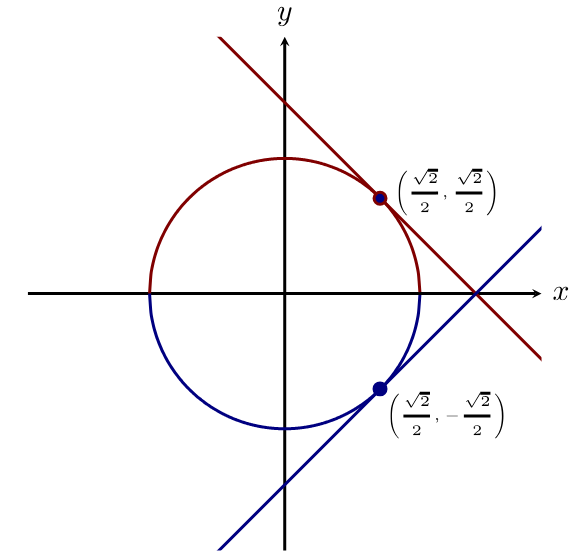
\includegraphics{2.png}
\end{image}



\end{example}


\begin{example}
  Find where the circle, defined by $x=\cos( t)$ and $y=\sin( t)$ on
  $[0,2\pi)$, has vertical and horizontal tangent lines.
  \begin{explanation}
    We compute the derivative 
    \[
    \dd[y]{x} = \frac{y'(t)}{x'(t)} = \answer[given]{-\frac{\cos t}{\sin t}}.
    \]
    The derivative is $0$ when $\cos( t)= \answer[given]{0}$. Note that we only need the values of $t$ in the interval $[0, 2\pi)$ that satisfy $\cos(t)$. 
    This  happens when $t=\pi/2$, and $t= 3\pi/2$. These two $t$ values correspond to the points $(0,1)$ and $(0,-1)$ on the circle.

    The normal line is horizontal (and hence, the tangent line is
    vertical) when $\sin t=\answer[given]{0}$. This happens when $t=
    0$ and $t=\pi$ corresponding to the points $(-1,0)$ and
    $(0,1)$ on the circle. These results should make intuitive sense.
  \end{explanation}





\end{example}

\begin{example}

Consider the parametric equations 

\[ 
\begin{cases}
x(t)&=\sin(2t) \\
y(t)&=\cos(3t)
\end{cases}
\]

Below is the curve traced out by the above parametric curves as $t$ varies over $[0, 2\pi)$. 

\begin{image}
  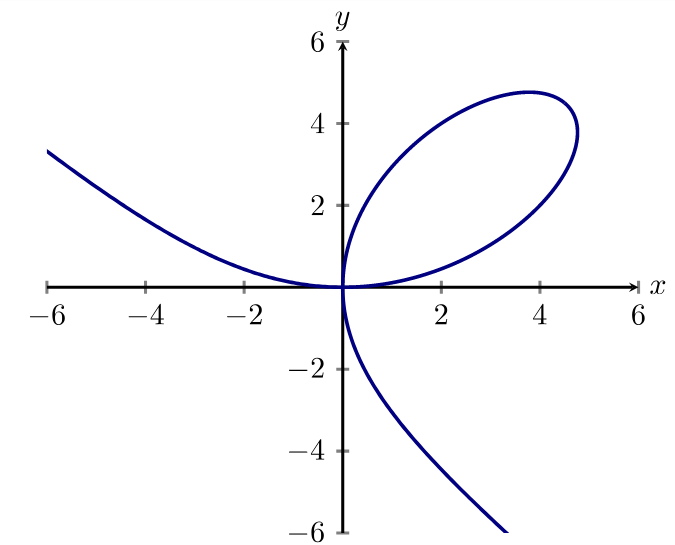
\includegraphics{3.png}
\end{image}

Notice that the origin belongs to the curve. What is the tangent line to the curve when at the origin?  Phrased in this manner, this question does not make sense. If we zoom in on
the origin, the curve does not begin to look more and more like a straight line. In fact, it will look like two lines crossing no matter how far we zoom in. Thus it seems that the curve is not differentiable at the origin. However we are only focusing on the curve itself rather than how the curve is traced out. Let's use the parametrization to investigate how the curve is traced out. 

The $t$ values for which the curve passes through the origin are obtained by find the $t$ values that simulaneously solve $\cos(3t)=0$ and $\sin(2t)=0$. 
This gives us $t=\pi/2$ and $t=9\pi/6$. 

See below how the curve is traced out as $t$ varies. Use the slider for $a$ to traced out the curve. 


\desmos{kffagvek2c}{1024}{500}


What is the tangent line to the curve when $t=\frac{\pi}{2}$? What about when $t=\frac{9\pi}{6}$. Look at the interactive figure below. Think of the parameter $t$ as time. Then the figure below shows a point corresponding to the time as well as some points corresponding to both future and past time values close to the given time. We see that if we look our curve for times close to $\frac{\pi}{2}$ we see that the curve looks approximately like a line. Similarly, if we look at our curve for times close to $\frac{9\pi}{6}$ then again we see that the curve looks approximately linear if we zoom in on the origin.

\desmos{girdw5krf7}{1024}{500}




 Now we can find the tangent line to the curve at the two different times it passes through the origin. 
Apply the formula 


\[
\frac{\d y}{\d x} = \frac{ y'(t)}{x'(t)}
\]

we get 
\[
\dd[y]{x}=\frac{\answer[given]{-3\sin(3t)}}{\answer[given]{2\cos(2t)}}
\]


Then calculating the $\dd[y]{x}$ when $t=\frac{\pi}{2}$ gives us $\answer[given]{ \frac{-3}{2}  }$. Thus the tangent line to the curve when $t=\frac{\pi}{2}$ is 
$y-\answer[given]{ 0}=\answer[given]{\frac{-3}{2}}(x-\answer[given]{0})$ (shown in orange below). 

Similarly the tangent line to the curve when $t=\frac{9\pi}{6}$ is $y-\answer[given]{0}=\answer[given]{\frac{3}{2}  }(x-\answer{0})$ (shown in green below).


\begin{image}
  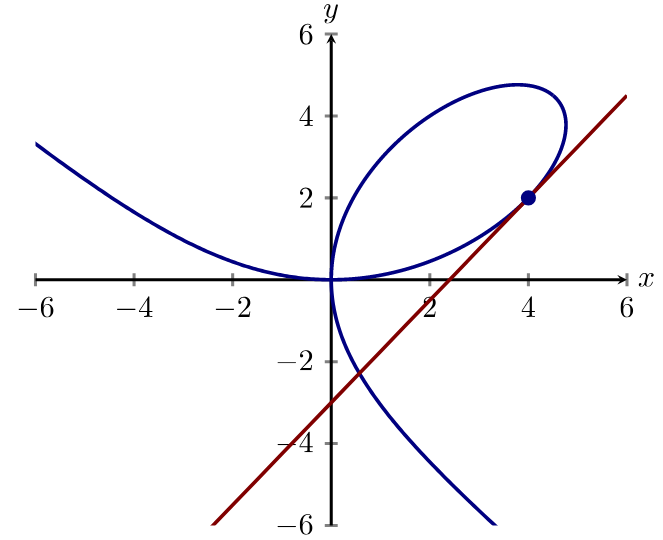
\includegraphics{4.png}
\end{image}



Finally here is a visualization that shows how the tangent line to the curve varies as we vary $t$. 

\desmos{l3efqzndog}{1024}{500}

\end{example}



%\section{Integrals}
%
%
%Assuming that the curve given by a parametric formula $(x(t),y(t))$
%represents $y$ as a function of $x$, that is traced out exactly once,
%we can integrate our parametric formula without too much additional
%trouble.  Again, recall that
%\[
%\d x = x'(t) \d t
%\]
%So we may write
%\[
%\int_a^b y \d x = \int_\alpha^\beta y(t) \cdot x'(t) \d t
%\]
%where $x(\alpha) = a$ and $x(\beta) = b$.
%
%We'll be talking about this in more detail soon, so a simple example
%should suffice.
%
%\begin{example}
%  Let $x(t) = \cos(t)$ and $y(t)= \sin(t)$ as $t$ runs from $0$ to
%  $\pi$:
%  \begin{image}
%    \begin{tikzpicture}
%      \begin{axis}[
%          xmin=-1.2,xmax=1.2,ymin=-.2,ymax=1.2,
%          axis lines=center,
%          xlabel=$x$, ylabel=$y$,
%          unit vector ratio*=1 1 1,
%          every axis y label/.style={at=(current axis.above origin),anchor=south},
%          every axis x label/.style={at=(current axis.right of origin),anchor=west},
%        ]        
%        \addplot [very thick, penColor, smooth, domain=(0:180)] ({cos(x)},{sin(x)});
%      \end{axis}
%    \end{tikzpicture}
%  \end{image}
%  Compute the area between this region and the $x$-axis on the
%  interval $[-1,1]$.
%  \begin{explanation}
%    We would like to compute:
%    \[
%    \int_{-1}^1 y \d x
%    \]
%    The parametric equations allow us to make a substitution: 
%    \begin{align*}
%      y(t) &=\answer[given]{\sin(t)}\\
%      \d x &=\answer[given]{-\sin(t)}\d t
%    \end{align*}
%    now then integral becomes
%    \[
%    \int_{-1}^{1} y \d x= \int_\alpha^\beta (\sin(t))(-\sin(t))\d t
%    \]
%    Now we need to find $\alpha$ and $\beta$. Note that using
%    \[
%    x(t)=\cos(t)
%    \]
%    When $x=-1$, $t=\answer[given]{\pi}$. Likewise, when $x=1$, $t=\answer[given]{0}$. Hence our
%    integral becomes
%    \begin{align*}
%      \int_{-1}^{1} y \d x&= \int_\pi^0 (\sin(t))(-\sin(t))\d t\\
%      &= \int_{\answer[given]{0}}^{\answer[given]{\pi}}\sin^2(t)\d t\\
%      &= \int_0^\pi\frac{1-\cos(2t)}{2}\d t\\
%      &= \int_0^\pi\frac{1}{2}-\frac{\cos(2t)}{2}\d t\\
%      &= \eval{\frac{t}{2}-\frac{\sin(2t)}{4}}_0^\pi\\
%      &= \answer[given]{\frac{\pi}{2}}
%    \end{align*}
%  \end{explanation}
%\end{example}



\end{document}






